%!TEX root = ../Masterthesis.tex
\begin{titlepage}

\begin{center}
\begin{figure}[!ht]
	\centering
		\includegraphics[width=\textwidth]{images/th_color_bar.png}
\end{figure}
\end{center}
%Deutscher Titel
\begin{flushleft}
\begin{Large}
Masterthesis Medientechnolgie\\
\end{Large}
\vspace{0.5cm}
\begin{LARGE}
\textbf{RHOT-A real-time hand and object tracking system with low cost consumer grade hardware}
\end{LARGE}
\end{flushleft}
\vspace{1.0cm}
\begin{flushleft}
\begin{Large}
vorgelegt von\\ 
\vspace{0.3cm}
\begin{LARGE}
\textbf{Oliver Kalbfleisch} \\
\end{LARGE}
\end{Large}
\end{flushleft}
\vspace{2.0cm}
\begin{flushleft}
\begin{Large}
Erstgutachter: Prof. Dr. Arnulph Fuhrmann(TH Köln) \\[1.0em]
Zweitgutachter: Prof. Dr. Stefan Michael Grünvogel(TH Köln)
\end{Large}
\end{flushleft}
\vspace{1.5cm}
\begin{flushleft}
\begin{large}
Juni \the\year
\end{large}
\end{flushleft}
\begin{figure}[!ht]
\begin{flushright}
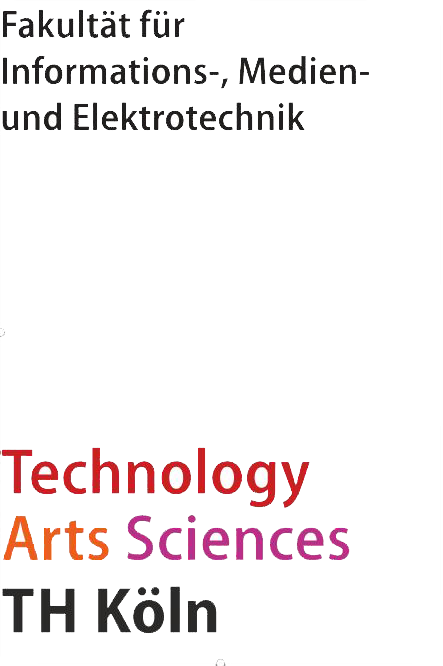
\includegraphics[width=0.25\textwidth]{images/TH_bottom_logo.png}
\end{flushright}
\end{figure}
\newpage
\setcounter{page}{1}
\pagenumbering{gobble}
\huge\textbf{Masterarbeit}\\\\
\large
Titel: RHOT Ein echtzeit Hand- und Objektrackingsystem basierend auf kostengünstiger Hardwarekomponenten\\
\textbf{Gutachter}:\\
	Prof. Dr. Arnulph Fuhrmann (TH Köln)\\
	Prof. Dr. Stefan Michael Grünvogel (TH Köln)\\
	\todo{übersetzen}
Zusammenfassung:\\ This paper will evaluate if it is possible to build a hand and object tracking system on low cost consumer grade hardware components. To keep system cost low, a set of Raspberry Pi's with the matching camera is used for image acquiring an processing. These processing units are linked to a master unit which takes care of stereoscopic depth calculations, the position value processing and the final rendering of a hand and object model in digital space. Several forms of colored marker types are assessed for the prototype application and compared in terms of tracking precision and limiting factors in terms of haptic restrictions for the fingers. The final results show that it is possible to achieve a tracking system solution with the used hardware components that has a suitable tracking update frequency and precision.\\
\textbf{Stichwörter}: Echtzeit,Inverse Kinematik, Hand-tracking, color-tracking,Objekt-tracking, günstig)\\
\textbf{Sperrvermerk}: (optional) Die Einsicht in diese Arbeit ist bis zum TT. Monat JJJJ gesperrt.\\
\textbf{Datum}: TT. Monat JJJJ\\
\newpage
\huge \textbf{Masters Thesis}\\\\
\large
\textbf{Title}: RHOT A real time hand and object tracking system with low cost consumer grade\\
\textbf{Reviewers}:\\
	Prof. Dr. Arnulph Fuhrmann (TH Köln)\\
	Prof. Dr. Stefan Michael Grünvogel (TH Köln)\\
\textbf{Abstract}: \\This paper will evaluate if it is possible to build a hand and object tracking system on low cost consumer grade hardware components. To keep system cost low, a set of Raspberry Pi's with the matching camera is used for image acquiring an processing. These processing units are linked to a master unit which takes care of stereoscopic depth calculations, the position value processing and the final rendering of a hand and object model in digital space. Several forms of colored marker types are assessed for the prototype application and compared in terms of tracking precision and limiting factors in terms of haptic restrictions for the fingers. The final results show that it is possible to achieve a tracking system solution with the used hardware components that has a suitable tracking update frequency and precision.\\
\textbf{Keywords}: Hand-tracking, Object-tracking, inverse kineamtics, low-cost, realtime \\
\textbf{Date}: 29 June 2018\\

\end{titlepage}
